\documentclass[10pt, nofootinbib, twocolumn]{revtex4-1}
\usepackage{amsmath}
\usepackage{xparse}
\usepackage{graphicx}
\usepackage{hyperref}
\usepackage{color}
\usepackage{physics}
\usepackage{enumitem}
\usepackage{natbib}
\usepackage{booktabs}
\usepackage{float}
\usepackage{caption}
\hypersetup{
    colorlinks=true,
    linkcolor=black,  
    citecolor=black,
    urlcolor=blue
}

\begin{document}
\vspace*{5\baselineskip}
\title{The Two-Dimensional Time-Dependent Schrodinger Equation} 
\author{Tiril Sørum}\homepage{https://github.com/tirilsg/FYS3150-Project5}
\date{\today}        
\begin{abstract}
\vspace*{1\baselineskip}
    \textit{The two-dimensional, time-dependent Schrodinger equation describing a wave-function is discretized in this report, and by utilizing \textit{the Crank-Nicolson Scheme}, we simulate how the behaviour of the wave-function evolves and changes with time. By creating different environments in which these wave-functions, modelling Gaussian wave-packets and thereby photons, interact with a wall containing an arbitrary amount of slits, we prove wave-particle duality. The correctness of our model is checked by first checking the standard deviation and relative error when modelling the wave packets in both an environment with no wall, and a wall containing double slits, we find relative errors on the minuscule scale of $10^{-15}$ and $10^{-14}$. Subsequently, simulations of the behaviour when interacting with a wall containing single, double and triple slits are carried out, and we find patterns in the demeanor only explained by important properties of waves, such as interference, thereby proving the wave-particle duality. These discoveries are made by visualizing the data accumulated from these simulations in the forms of GIFs and probability-density plots. }
\end{abstract}
\maketitle       

\section{Introduction}\label{sec:introduction}
The discovery of wave-particle duality is a crucial concept in quantum mechanics, significantly improving our understanding of how quantum entities behave. This concept entails an explanation for the behaviour of quantum entities, by a possession of both particle and wave properties. \\

Light is electromagnetic radiation, consisting of particles known as photons. An extremely important characteristic of the photon, is that it does in fact possess wave-particle duality, as we can model it as both a particle with quantized energy, or as energy packets \cite{kvante}. \textit{"If light can behave like a stream of particles, then perhaps it is not so surprising that electrons can behave like waves \cite{thermal}."}\\

To investigate this statement, we implement a model predicting the behaviour of wave-packets within a restricted, defined environment, in which collision between these wave-packets and a wall occurs. This wall contains an arbitrary amount of slits, in which waves can pass through. Particles passing through slits in a wall like this, will exhibit a behaviour in which the particle interferes with itself \cite{kvante}. This is a pattern of behaviour that is directly observable, by simulating such an interaction, that we call the \textit{Double Slit Experiment}. \\

\vspace*{1\baselineskip}
To be able to describe the behaviour, and the interference pattern expected to occur, we need to introduce both wave-functionality, and thereby \textit{the Schrödinger equation}, which describes the behaviour of the wave function. \\

By creating a model for this experiment, commonly undergone by making use of a double slit setup, which is what we do, and investigating the observed behaviour, we confirm and visualize these characteristics of wave-particle duality. Simulations are ran for both the behaviours for no slits, one slit, double slits and triple slits in the wall, and the results are presented in both Figures and GIFs presented in this report. We discuss the results in accordance with our theory, and find a striking conformity, proving the wave-particle duality.




\clearpage
\section{Theory}\label{sec:theory}
\subsection{Expected Behaviours}\label{sec:behaviour}
Waves behave in accordance with two extremely important properties of waves ; \textit{Huygens principle} and the \textit{superposition principle}.

\subsubsection{Huygens Principle}
\textit{Huygens principle} \cite{oscillations} states that \textit{"any point on a wave can be viewed as a source of a new wave, called the elementary wave, which expands in all directions."} In practice, this implies that each point along a wavefront can be seen as a secondary source of waves, contributing to the overall propagation of the wave. This principle is an important explanation as to the behaviour of waves when interacting with its environment. 

\subsubsection{Superposition Principle}
The \textit{superposition principle} \cite{oscillations}, states that \textit{"the response to two or more concurrent stimuli will at a given time and place be equal the sum of the response the system would have on each of the stimuli individually."}. When applied to waves, this principle implies that the combined effect of multiple waves at a given point in space and time, is the sum of their individual effects. When seen in light of Huygens principle, it is clear that the appearance of wave fronts will depend on the sum of every wavelet constructed along a wavefront. 


\subsubsection{Interference}
The phenomena which describes whether waves combine to reinforce of cancel each other, is commonly referred to as interference. When two waves coincide, the interference is constructive and the intensity in these regions increase as a consequence of the amplitudes of the wave functions adding up. When these amplitudes subtract, the interference is destructive and the intensity becomes lower. This is reason to distinct patterns forming where such waves cross paths. 


\newpage
\subsection{The Wave Function}
The Schrödinger equation is used to describe the behaviour of wave functions and wave-packets, and predicts the future behaviour of a dynamic system, in form of probability for these behaviours to occur, and is dependent on both real and imaginary numbers. The most general form of this important equation, is time-dependent, and expressed by 
\begin{equation}\label{eq:schrr}
    i \hbar \frac{d}{dt} |\Psi(t)\rangle = \hat{H} |\Psi(t)\rangle
\end{equation}
where $\hbar$ is Planck's constant, t is time, $|\Psi(t)\rangle$ is in the shape of a vector and describes the quantum state of our system, and $\hat{H}$ is referred to as the \textit{Hamiltonian operator}. The  \textit{Hamiltonian operator} corresponds to the total energy within the system of interest, which due to its shape, keeps the energy real. For a system which is located in an environment affected by a potential $V$, and is not affected by an external magnetic field, $\hat{H}$ becomes \cite{griffiths}
\begin{equation}\label{eq:hamiltonian}
    \hat{H}=-\frac{\hbar^2}{2m}\nabla^2 +V_0
\end{equation}
where m is the mass of the respective particle with a condition modelled by the operator, $V_0$ is the  potential. $\nabla^2$ is the \textit{Laplace operator}, and has the shape of 
\begin{equation}\label{eq:laplace}
    \nabla^2= \frac{\partial^2}{\partial x^2}+ \frac{\partial^2}{\partial y^2}+ \frac{\partial^2}{\partial z^2}
\end{equation}
By making use of these Equations \eqref{eq:hamiltonian} and \eqref{eq:laplace}, the time-dependent Schrödinger Equation \eqref{eq:schrr} becomes
\begin{equation}\label{eq:schrlar}
    i \hbar \frac{d}{dt} |\Psi(t)\rangle = (-\frac{\hbar^2}{2m}(\frac{\partial^2}{\partial x^2}+ \frac{\partial^2}{\partial y^2}) +V_0) |\Psi(t)\rangle
\end{equation}
$|\Psi(t)\rangle$ is commonly referred to as the \textit{wave function}, and can be expressed $\Psi(x,y,t)$. \\

\textit{The Born rule} conveys the probability of finding a system in a certain condition - a certain position in the pertinent space at a certain time. Thereby, this postulate of quantum mechanics can be referred to as the probability density \cite{thermal} - or distribution, expressed by the Equation \eqref{eq:problar}
\begin{equation}\label{eq:problar}
    p(x,y\,;t) = |\Psi(x,y,t)|^2 = \Psi^*(x,y,t) \, \Psi(x,y,t)
\end{equation}
which is a positive, real number as a consequence of our expression, relying on both the wave function and its complex conjugate. \\



\newpage
\section{Methods}\label{sec:methods} 
\subsection{Simplification of the Wave Function}
In the specific context of efficient simulation using these complex equations, an assumption of scaling dimensional variables away successfully is made. As a consequence of this assumption, the expressions for the Schrödinger Equation \eqref{eq:schrr} and the associated probability distribution Equation \eqref{eq:problar} becomes 
\begin{equation}\label{eq:schr}
    i \frac{\partial u}{\partial t} = -\frac{\partial^2 u}{\partial x^2} - \frac{\partial^2 u}{\partial y^2} + v(x,y) u.
\end{equation}
\begin{equation}\label{eq:prob}
    p(x,y;t) = |u(x,y,t)|^2 = u^*(x,y,t) \, u(x,y,t)
\end{equation}
where $u(x,y,t)$ is the wave function and describes position in time and space, and $v(x,y)$ describes the potential in which the system remains. These expressions are only possible to deduce, on the assumption that $u(x,y,t)$ has been normalised \cite{griffiths} - the following condition is reached
\begin{equation}\label{eq:norm}
    \int_{\infty}^{\infty}{u^*(x,y,t) \, u(x,y,t)} \, = \, 1
\end{equation}
By implementing these dimensionless equations Equation \eqref{eq:schr} and Equation \eqref{eq:prob}, a wave function and boundary conditions that are subsequently simple can be derived for the system. 

\subsection{Boundary Conditions}
The lack of dimensions leaves a description of the two dimensional xy-space in as intervals $x\epsilon[0,1]$, $y\epsilon[0,1]$. We know that as these boundaries in the xy-plane are approached, the wave function approaches 0, and thereby
\begin{align}\label{eq:dirich}
    \begin{split}
        u(x=0,y,t)=0 \\
        u(x=1,y,t)=0 \\
        u(x,y=0,t)=0 \\
        u(x,y=1,t)=0 \\
    \end{split}
\end{align}
This way, one manages to avoid a large scale operation as $x,y \longrightarrow \infty$, as boundaries are applied to the wave function. These boundary conditions expressed by Equation \eqref{eq:dirich} is normally referred to as Dirichlet conditions \cite[p. ~333]{notes} for a square lattice with initial condition, for an unnormalised Gaussian wave packet
\begin{equation}\label{eq:init}
    u(x,y,t=0) = e^{-\frac{(x-x_c)^2}{2 \sigma_x^2} - \frac{(y-y_c)^2}{2 \sigma_y^2} + i p_x x + i p_y y}
\end{equation}
where $\sigma_x$ and $\sigma_y$ refers to the initial standard deviation in both dimensions, $p_x$ and $p_y$ are the initial momentum of the wave packet in the respective directions - which can be derived from our Hamiltonian operator's expression of kinetic energy, and $x_c$ and $y_c$ are the initial coordinates of the centre of the wave packet in the two dimensional space. The expression for the wave function of a Gaussian wave packet is applicable to the case of photon-behaviour, and thereby Equation \eqref{eq:init} can be utilized as the initial condition for such a system. 



\subsection{Numeric Solution to the Wave Function}
\subsubsection{Discretization of System}
Furthermore, discretization of the scaled Schrödinger Equation \eqref{eq:schr} is utilized, to further derive a numeric solution for the wave function. This is done by first constructing a two-dimensional spacial grid of M points in both x- and y-directions, with constant step-size $h=\Delta x = \Delta y$ between each of these points. The grid is expressed by coordinates $x_i$ and $y_j$
where i and j are be used to navigate the points in the grid, and are subsequently real integers. The Dirichlet conditions expressed by Equations \eqref{eq:dirich} are applied to this space, so 
\begin{align}
    \begin{split}
        x_i=ih \, , i \, \epsilon \, \{1,2,...,M-2\} \\
        y_j=jh \, , j \, \epsilon \, \{1,2,...,M-2\} \\
        t_n = n\Delta t \, , n \, \epsilon \, \{0,1,2,...,N_t\}  \\
    \end{split}
\end{align}
where $t_n$ is the discretized time, with a constant step in time $\Delta t$, for a total time $T=N_t$. Both the scaled Schrödinger Equation \eqref{eq:schr} and probability distribution Equation \eqref{eq:prob} can be expressed in these discretized terms
\begin{equation}\label{eq:schrdis}
    i \frac{\partial}{\Delta t} u^n_{i,j}= -(\frac{\partial^2 }{\partial x^2} - \frac{\partial^2 }{\partial y^2})u^n_{i,j} + v(x,y) u^n_{i,j}
\end{equation}
\begin{equation}\label{eq:probdis}
    p(x_i,y_i;t_n) = u^{n*}_{i,j} \, u^n_{i,j}
\end{equation}
Thereby, the entire space in which the wave-function is allowed to exist, can be defined at the different points in the grid, and as a consequence also the wave-behaviour expression is defined at these points.


\subsubsection{Crank-Nicolson Scheme}\label{sec:crank}
To be able to estimate the behaviour of the wave-function as time passes, a method needs to be implemented. 
\textit{The Crank-Nicolson Scheme} estimates the discretized wave-function by combining the methods we know as Forward- and Backward Euler. Since \( u_{i,j}^n \) represents the wave function at the grid point \( (x_i, y_j, t_n) \), and by letting \( F_{i,j}^n \) be an operator defined as
\begin{equation}\label{eq:probdis}
    F_{i,j}^n = i \frac{\partial}{\Delta t} u^n_{i,j}= -(\frac{\partial^2 }{\partial x^2} - \frac{\partial^2 }{\partial y^2})u^n_{i,j} + v(x,y) u^n_{i,j}
\end{equation}
the expression for Crank-Nicolson is derived by first taking a look at Forward and Backward-Euler:\\
The \textit{Forward Euler} expression for \( F_{i,j}^n \) is given by \cite{notes}: \\
\begin{equation}\label{eq:forward}
    \begin{split}
        F_{i,j}^n = i \frac{u^{n+1}_{i,j}-u^{n}_{i,j}}{\Delta t} \\
        -\frac{u^n_{i+1,j}-2u^n_{i,j}+u^n_{i-1,j}}{h^2} \\
        - \frac{u^n_{i,j+1}-2u^n_{i,j}+u^n_{i,j-1} }{h^2} + u^n_{i,j}v_{i,j}
    \end{split}
\end{equation}

The \textit{Backward Euler} expression for \( F_{i,j}^n \) is given by \cite{notes}: \\
\begin{equation}\label{eq:backward}
    \begin{split}
        F_{i,j}^{n+1} = i \frac{u^{n+1}_{i,j}-u^{n}_{i,j}}{\Delta t} \\
        -\frac{u^{n+1}_{i+1,j}- 2u^{n+1}_{i,j}+u^{n+1}_{i-1,j}}{h^2} \\ -  \frac{u^{n+1}_{i,j+1}-2u^{n+1}_{i,j}+u^{n+1}_{i,j-1} }{h^2} + u^{n+1}_{i,j}v_{i,j}
    \end{split}
\end{equation}

Taking the advantage of the Forward and Backward Euler expressions, we get the \textit{Crank-Nicolson Scheme} \cite{notes}: 
\begin{equation}\label{eq:crank}
    \begin{split}
        i \frac{u^{n+1}_{i,j}-u^{n}_{i,j}}{\Delta t} = \frac{1}{2}(F_{i,j}^n+F_{i,j}^{n+1})  
    \end{split}
\end{equation}

This expression is subsequently utilized to retrieve an expression for the discretized wave-function as it evolves in time. The following expression for discretized Schrödinger Equation is retrieved: 
\begin{equation}\label{eq:wave}
    \begin{split}
        u_{ij}^{n+1}  -  r \left[u_{i+1,j}^{n+1} - 2u_{ij}^{n+1} + u_{i-1,j}^{n+1}\right]  - \\
        r \left[u_{i,j+1}^{n+1} - 2u_{ij}^{n+1} + u_{i,j-1}^{n+1}\right]  +  \frac{i \Delta t}{2} v_{ij} u_{ij}^{n+1} \\
        = u_{ij}^n  +  r \left[u_{i+1,j}^n - 2u_{ij}^n + u_{i-1,j}^n\right]  +  \\ 
        r \left[u_{i,j+1}^n - 2u_{ij}^n + u_{i,j-1}^n\right]  -  \frac{i \Delta t}{2} v_{ij} u_{ij}^n,
    \end{split}
\end{equation}
where $r = \frac{i \Delta t}{2 h^2}$. The deduction of this expression can be viewed in the Appendix. \ref{sec:appendix}. \\

The errors of computation when making use of the Crank-Nicolson Scheme is described \cite[p. ~312]{notes} $O(\Delta x^2)$ and $O(\Delta t^2)$, which indicates a good degree of precision, and stability for both $\Delta x$ and $\Delta t$. This formulation allows for the efficient estimation of the behaviour of wave-functions using standard linear algebra techniques. \\


\subsection{Implementation of Model}\label{sec:implementation}
We wish to create a simulation, which visualizes the interaction between the wave-packets and a wall containing an arbitrary amount of slits, an example visualized in Figure \ref{fig:example}. To do so, we need to implement a function which helps us model this wall, and thereby also behaviour of the wave-function before, during and after interaction. We do this by initializing the system's potential in the two-dimensional xy-space. By setting the potential high where we wish to create barriers, we manage to create a simple model for a wall with arbitrary thickness, position in the xy-space, as well as amounts of slits and their size. \\

\begin{figure}[H]
    \caption{Visualization of the \textit{Double Slit Experiment}, where waves are being sent towards a wall with two slits. Interference patterns appears as a consequence of this interaction. Figure retrieved from \cite[p.~426]{oscillations}.}
    \centering
    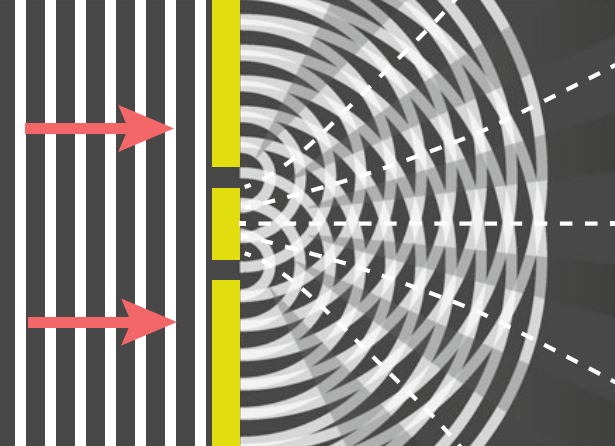
\includegraphics[width = 0.55\textwidth]{figures/interference.pdf} 
    \label{fig:example}
\end{figure} 
\subsubsection{Construction of Wall}\label{sec:wall}
As a general preset for the model of the wall, we make use of the following settings for a double slit setup:
\begin{center} ------------------------------------------------------------ \end{center}
\begin{description}[]
    \item \textbf{Wall thickness in the $x$ direction:} 0.02
    \item \textbf{Wall position (centre) in the $x$ direction:} 0.5
    \item \textbf{Length of the wall piece separating the two slits:} 0.05
    \item \textbf{Slit aperture (opening in the $y$ direction):} 0.05 
    \item \textbf{Ensure symmetry around $y = 0.5$:} For a double-slit, the wall piece separating the two slits should be centered on $y = 0.5$.
\end{description}
\begin{center} ------------------------------------------------------------ \end{center}
When constructing walls containing more than one slit, we make sure to center the slits around the middle of the wall, so that the spacing between each slit is consistent, and the setup is mirrored in the y-axius over y=0.5.

\newpage
\subsubsection{Algorithm}\label{sec:algorithm} 
Implementations of a couple other functions is required, for the model to be suited for simulations. We implement functions that initialize our system, including the initial state of our wave function. Furthermore, functions needed to make use of the algorithm presented for he Crank-Nicolson Scheme to estimate the behaviour of our wave packets, as well as the algorithm itself are actualized. Simulations are ran by calling the Crank-Nicolson Scheme to model behaviour for an arbitrary amount of steps in time, during an interval in time $T$ we see fit. This is done by making use of matrices expressing our discretized space. \\

The Equation \eqref{eq:wave} can be expressed in terms of matrices, with consideration to relevant boundary conditions, by the Equation \eqref{eq:matrices}:
\begin{equation}\label{eq:matrices}
    A \,\vec{u}^{n+1} = B \,\vec{u}^{n}
\end{equation}
where $\vec{u}^n$ and  $\vec{u}^{n+1}$ are column vector that contains $u^n_{ij}$ or $u^{n+1}_{ij}$ values for each point in our $(M-2)\times (M-2)$ grid, or xy-space, at a time characterized by the time step n and A and B are large traditional $(M-2)^2\times (M-2)^2$  matrices, constructed:
\[
A = 
\begin{bmatrix}
    \begin{bmatrix}     a_{k} & -r & 0 & 0 \\     -r & a_{2k} & \ldots & 0 \\     0 & \ldots & \ldots & -r \\     0 & 0 & -r & a_{(M-2)k} \end{bmatrix} & \begin{bmatrix}     -r & 0 & 0 & 0 \\     0 & -r & \ldots & 0 \\     0 & \ldots & \ldots & 0 \\     0 & 0 & 0 &-r \end{bmatrix} & 0  \\
    \begin{bmatrix}     -r & 0 & 0 & 0 \\     0 & -r & \ldots & 0 \\     0 & \ldots & \ldots & 0 \\     0 & 0 & 0 &-r \end{bmatrix}  & \ldots & \begin{bmatrix}     -r & 0 & 0 & 0 \\     0 & -r & \ldots & 0 \\     0 & \ldots & \ldots & 0 \\     0 & 0 & 0 &-r \end{bmatrix}  \\
    0 & \begin{bmatrix}     -r & 0 & 0 & 0 \\     0 & -r & \ldots & 0 \\     0 & \ldots & \ldots & 0 \\     0 & 0 & 0 &-r \end{bmatrix} & \begin{bmatrix}     a_{k} & -r & 0 & 0 \\     -r & a_{2k} & \ldots & 0 \\     0 & \ldots & \ldots & -r \\     0 & 0 & -r & a_{(M-2)k} \end{bmatrix} \\
\end{bmatrix}
\]

\[
B = 
\begin{bmatrix}
    \begin{bmatrix}     b_{k} & r & 0 & 0 \\     r & b_{2k} & \ldots & 0 \\     0 & \ldots & \ldots & r \\     0 & 0 & r & b_{(M-2)k} \end{bmatrix} &  \begin{bmatrix}     r & 0 & 0 & 0 \\     0 & r & \ldots & 0 \\     0 & \ldots & \ldots & 0 \\     0 & 0 & 0 &r \end{bmatrix} & 0\\
    \begin{bmatrix}     r & 0 & 0 & 0 \\     0 & r & \ldots & 0 \\     0 & \ldots & \ldots & 0 \\     0 & 0 & 0 &r \end{bmatrix}  & \ldots & \begin{bmatrix}     r & 0 & 0 & 0 \\     0 & r & \ldots & 0 \\     0 & \ldots & \ldots & 0 \\     0 & 0 & 0 &r \end{bmatrix}  \\
    0 &    \begin{bmatrix}     r & 0 & 0 & 0 \\     0 & r & \ldots & 0 \\     0 & \ldots & \ldots & 0 \\     0 & 0 & 0 &r \end{bmatrix} & \begin{bmatrix}     b_{k} & r & 0 & 0 \\     r & b_{2k} & \ldots & 0 \\     0 & \ldots & \ldots & r \\     0 & 0 & r & b_{(M-2)k} \end{bmatrix}  \\
\end{bmatrix}
\]
where $r = \frac{i \Delta t}{2 h^2}$, and \\
\( a_k = 1 + 4r + \frac{i \Delta t}{2} v_{i,j} \) \\ 
\( b_k = 1 - 4r - \frac{i \Delta t}{2} v_{i,j} \) \\

where k, for all these definitions, is an element in the interval $k\epsilon \{1,2,...,M-2\}$, and i refers to the complex number, not the index used to maneuver the matrices used in the previous deduction. This means, in practice, the matrices A and B contain other two-dimensional matrices, thereby describing a three dimensional space. This space is described by the dimensions x and y, as well as time t. \\

\cleardoublepage
This method can be implemented, as the algorithm:\\
\begin{center} ------------------------------------------------------------ \end{center}
\begin{description}[]
    \item \textbf{Set initial conditions}, including initial wave-function given by Equation \eqref{eq:init}.
    \item \textbf{Set up potential} \( v(x, y) \) which our system is located in, defined to model the wall described in Section \ref{sec:implementation}. 
    \item \textbf{Fill the matrices A and B} needed to make use of the Crank-Nicolson Scheme, according to Equation \eqref{eq:matrices} and theory presented in Section \ref{sec:crank}.
    \item \textbf{Loop that evolves} our system in time. For each time step:
    \begin{itemize}
        \item Compute  \( \vec{b} = B \vec{u}^n \)
        \item Solve \( A \vec{u}^{n+1} = \vec{b} \) $-$ Equation \eqref{eq:matrices} $-$ for \( \vec{u}^{n+1} \)
        \item Store \( \vec{u}^{n+1} \) and the probability distribution described by Equation
        \eqref{eq:probdis}
    \end{itemize}
\end{description}
For each loop, the calculated behaviour of the wave-function is used as foundation for the next calculation of behaviour. 
\begin{center} ------------------------------------------------------------ \end{center}


\subsection{Simulation}
In addition to simulating the waves hitting a wall containing two slits, we wish to run the same simulations for the instances of one and three slits. This is done by making changes to the parameters used to define the potential, and subsequently running simulations. The behaviour of our wave-packets is visualized by plotting the probability of measuring a particle at different positions within our system at different times. 

\newpage
\subsection{Tools}
Numerous tools need to be taken advantage of in order to perform simulations, and visualize these results adequately. 
The simulations are performed by making use of the c++ module "armadillo", which lets us perform matrice operations with ease. This lets us store the simulation data in cubes, a three dimensional space representing the two dimensional xy-space as it evolves in time. Furthermore, the c++ modules "complex" and "assert.h" are used to make use of complex numbers and operations, as well as verifying assumptions created by code. In python, the modules "numpy", "matplotlib.pyplot" and "matplotlib.animation" are used to define arrays and create plots and animations. The python module "scipy" is used to define the peaks of functions created by data imported using "pyarma". To make sure our plots remain as clean as possible, "mpl\_toolkits.axes\_grid1" is used to modify axes and plot sizes.\\

To maneuver through the different functionalities of these modules, as well as finding the correct modules to use, ChatGPT is used. This website is also useful to help both customizing the appearance of reports written in latex such as this one, and expression of equations and referencing these. When writing code, ChatGPT is also used for debugging and troubleshooting purposes. \\

Another tool utilized to make the coding process easier, is GitHub. The repository
\href{https://github.com/artmenlope/double-slit-2d-schrodinger}{repository} (https://github.com/artmenlope/double-slit-2d-schrodinger) models a double slit experiment in python, which works as a great help for the direction of the c++ model.


\cleardoublepage
\section{Results}\label{sec:results}
\subsection{No Barriers vs. Double Slits}
We initialize two systems with settings $h = 0.005$, $\Delta t = 2.5\times10^{-5}$, $T = 0.008$, $x_c = 0.25$, $\sigma_x = 0.05$, $p_x = 200$, $y_c = 0.5$, $\sigma_y = 0.05$ and $p_y = 0$. Thereby, each system is modelled with either no barriers, meaning the potential is $v_0=0$ within our entire system, or with a wall with two slits, with potential $v_0 = 1\times10^{10}$ and $\sigma_y = 0.10$, and other settings for the wall presented in section \ref{sec:implementation}. To compare the behaviour within these two systems, the deviation of the total probability from 1 as a function of time is visualized in Figure \ref{fig:prob7}.

\begin{figure}[H]
    \caption{Visualization of the deviation of the total probability from 1 as a function of time, for simulation of wave function behaviour with wall containing both no slits, and two slits. The double slits are defined by $v_0 = 1\times10^{10}$ and $\sigma_y = 0.10$.}
    \centering
    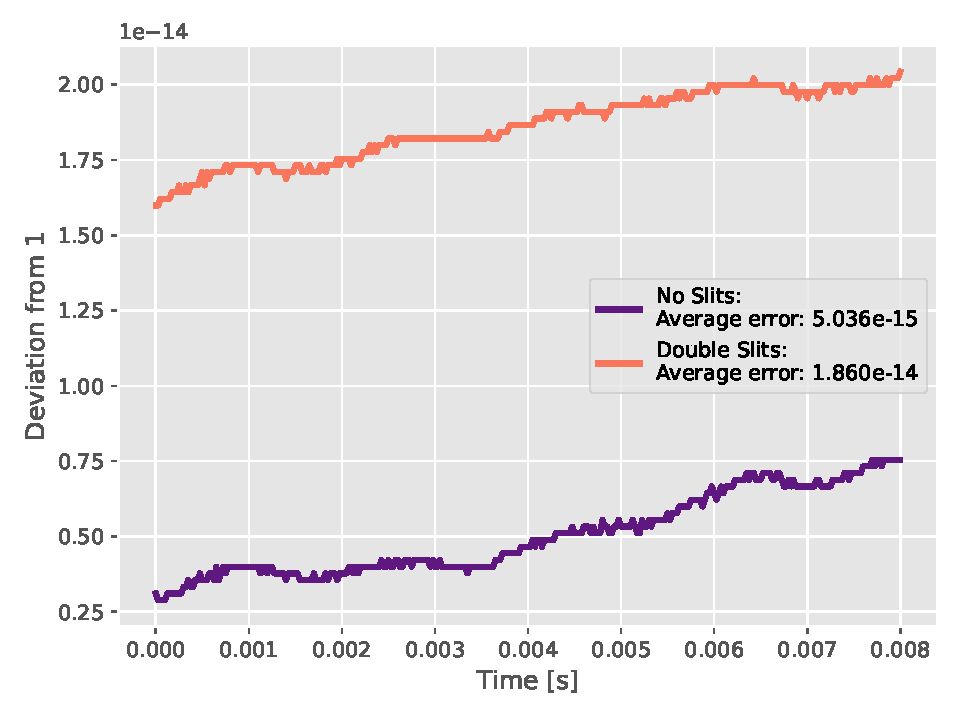
\includegraphics[width = 0.5\textwidth]{figures/deviation.pdf} 
    \label{fig:prob7}
\end{figure} 


\subsection{Double Slits}
The double slit settings presented in section \ref{sec:implementation} is used, in combination of an environment defined by the variable-settings $h = 0.005$, $\Delta t = 2.5\times10^{-5}$, $T = 0.002$, $x_c = 0.25$, $\sigma_x = 0.05$, $p_x = 200$, $y_c = 0.5$, $\sigma_y = 0.20$, $p_y = 0$ and $v_0 = 1\times10^{10}$ to simulate the behaviour of the wave-function when interacting with a wall containing two slits. The time evolution of the probability function in this simulation is illustrated in Figure \ref{fig:doubleprob}, at times t=0, t=0.001 and t=0.002. The same probability, divided into real and imaginary dimensions, is visualized in Figure \ref{fig:doubleprobre} and Figure \ref{fig:doubleprobim}. For the case of t=0.002, the probability in the xy-space is visualized in 3D, Figure \ref{fig:doubleprob3D}. 

\begin{figure*}
    \caption{Probability of measuring a particle at the different positions in the xy-plane, for a wall defined by two slits, at times t=0, t=0.001 and t=0.002.}
    \centering
    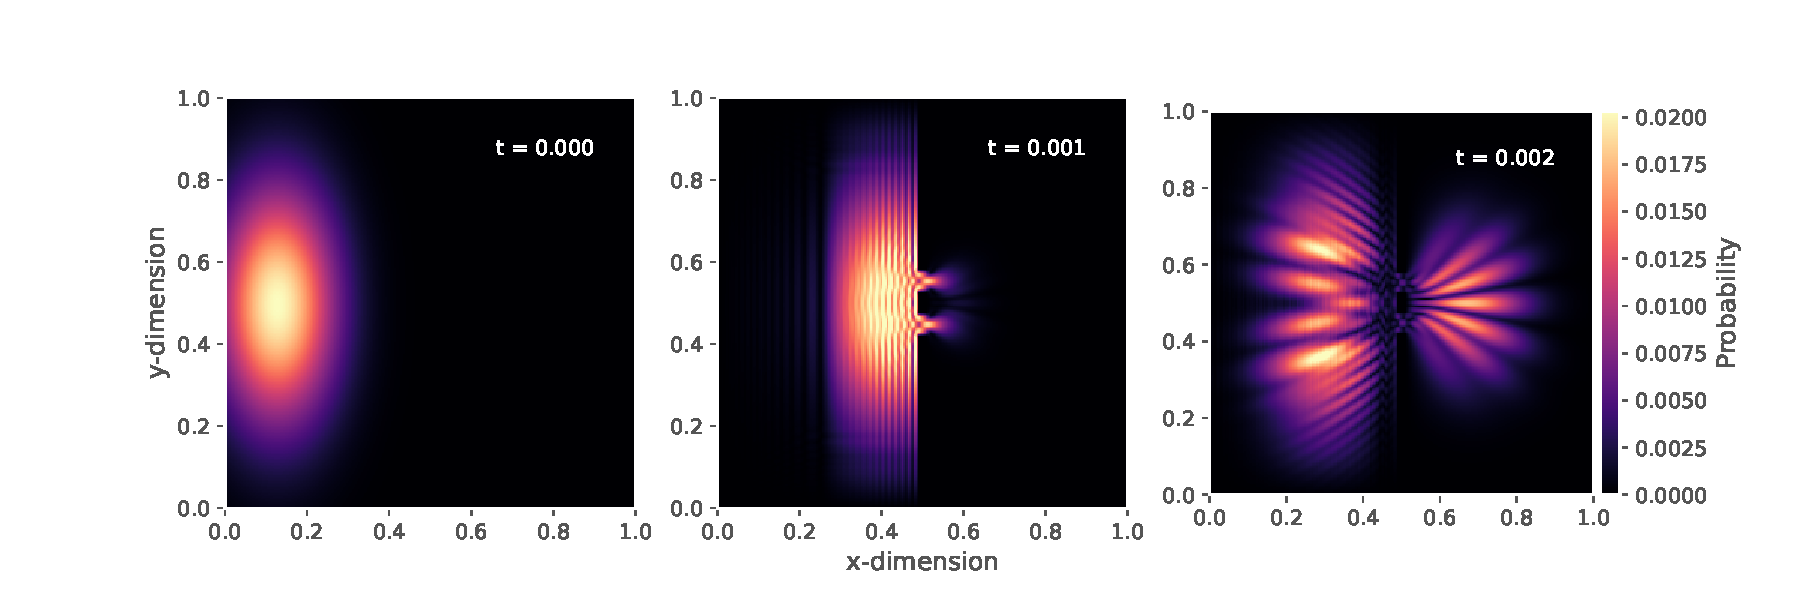
\includegraphics[width = 1\textwidth]{figures/plots_both.pdf} 
    \label{fig:doubleprob}
\end{figure*} 

\begin{figure*}
    \caption{Probability of measuring a particle at the different positions in the xy-plane, for a wall defined by two slits, at times t=0, t=0.001 and t=0.002. Only the real dimensions of the complex values.}
    \centering
    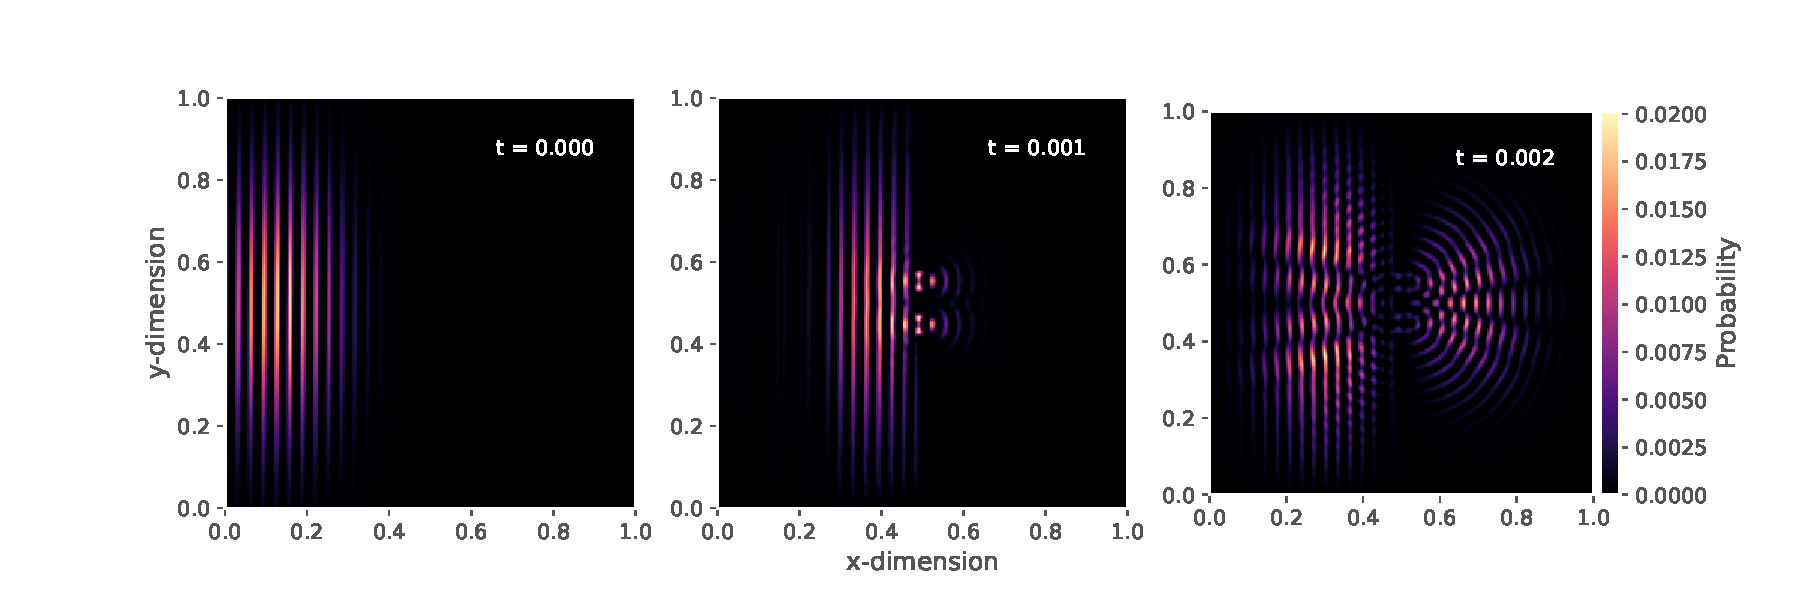
\includegraphics[width = 1\textwidth]{figures/plots_real.pdf} 
    \label{fig:doubleprobre}
\end{figure*} 

\begin{figure*}
    \caption{Probability of measuring a particle at the different positions in the xy-plane, for a wall defined by two slits, at times t=0, t=0.001 and t=0.002. Only the imaginary dimensions of the complex values.}
    \centering
    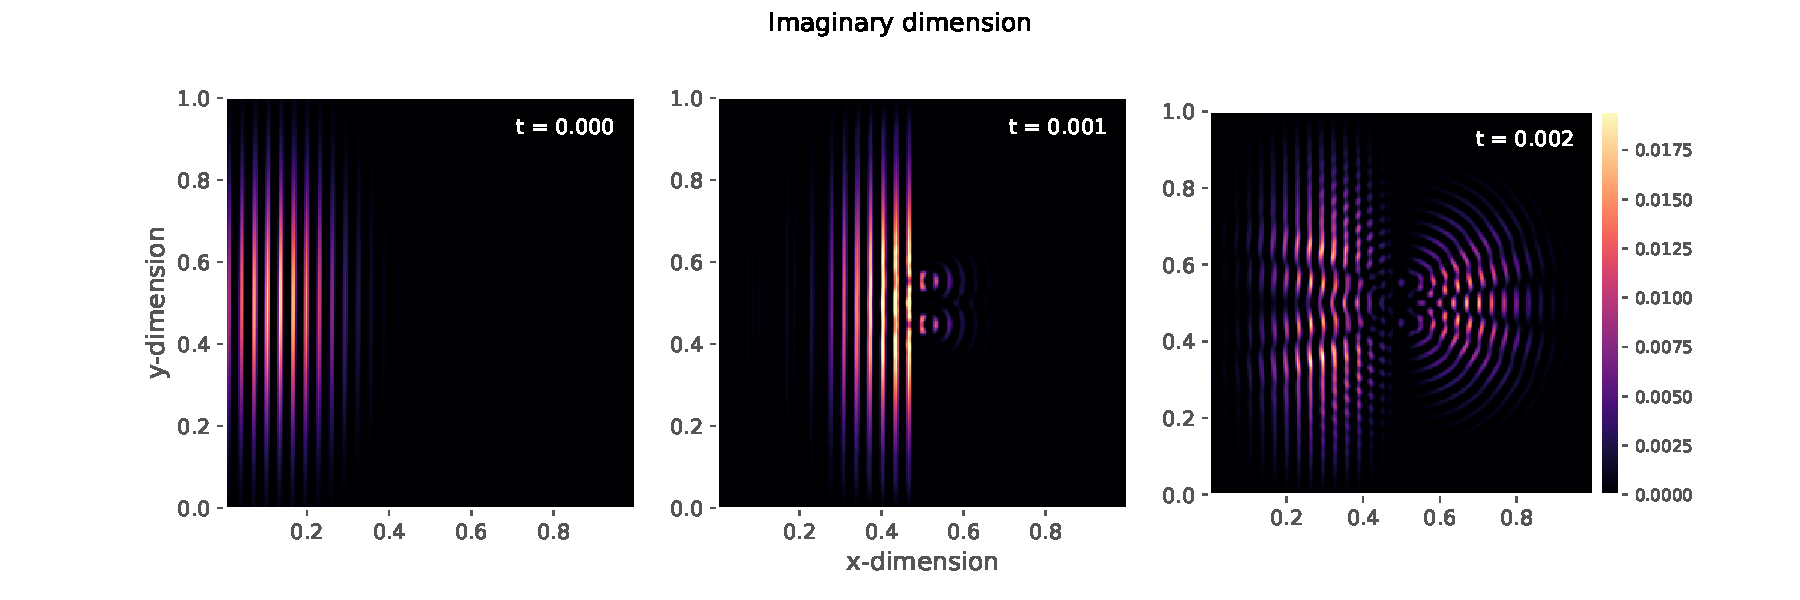
\includegraphics[width = 1\textwidth]{figures/plots_imag.pdf} 
    \label{fig:doubleprobim}
\end{figure*} 


\begin{figure}[H]
    \caption{Probability of measuring a particle at the different positions in the xy-plane, for a wall defined by two slits at time t=0.002 \textbf{in 3D}.}
    \centering
    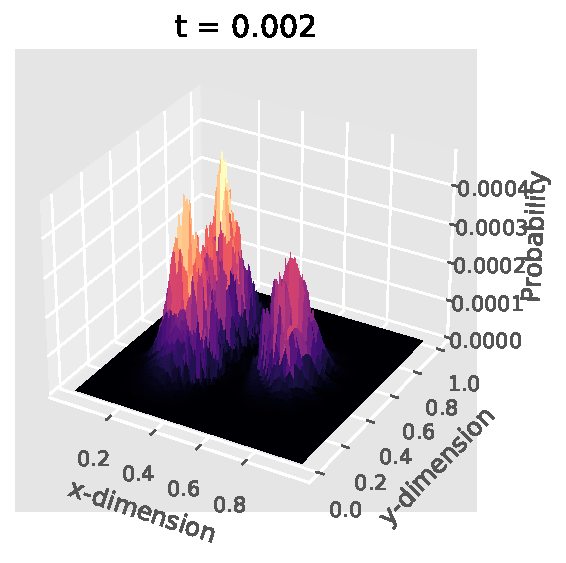
\includegraphics[width = 0.5\textwidth]{figures/plot_both_3d.pdf} 
    \label{fig:doubleprob3D}
\end{figure} 

Visualization of probability as a function of time in the shape of GIFs can be viewed by imgur-links in the Appendix, section \ref{sec:links}.



\subsection{Single Slit}
A single slit model is constructed by applying the same settings for potential as previously, adjusted for a single slit, as well as the settings for simulation and environment $h = 0.005$, $\Delta t = 2.5\times10^{-5}$, $T = 0.002$, $x_c = 0.25$, $\sigma_x = 0.05$, $p_x = 200$, $y_c = 0.5$, $\sigma_y = 0.20$, $p_y = 0$ and $v_0 = 1\times10^{10}$. Aperture is set to 0.05. Visualization of probability as a function of time in the shape of GIFs can be viewed by imgur-links in the Appendix, section \ref{sec:links}.



\subsection{Triple Slits}
A triple slit model is constructed by applying the same settings for potential as previously, adjusted for three slits, as well as the settings for simulation and environment $h = 0.005$, $\Delta t = 2.5\times10^{-5}$, $T = 0.002$, $x_c = 0.25$, $\sigma_x = 0.05$, $p_x = 200$, $y_c = 0.5$, $\sigma_y = 0.20$, $p_y = 0$ and $v_0 = 1\times10^{10}$. Aperture is set to 0.05 and walls of length 0.05 in y-dimensions is used to separate the slits. Visualization of probability as a function of time in the shape of GIFs can be viewed by imgur-links in the Appendix, section \ref{sec:links}.



\subsection{Detection Probability on Screen}
The data accumulated by simulating a single, double and triple slits is collected, and compared by visualizing the probability along the y-axis at position x=0.8 and time t=0.002 in the same figure, Figure \ref{fig:comparison}. 

\begin{figure}[H]
    \caption{Probability for discovering particles along the y-axis at position x=0.8 and time t=0.002. For the instances of one, two and three slits in the wall.}
    \centering
    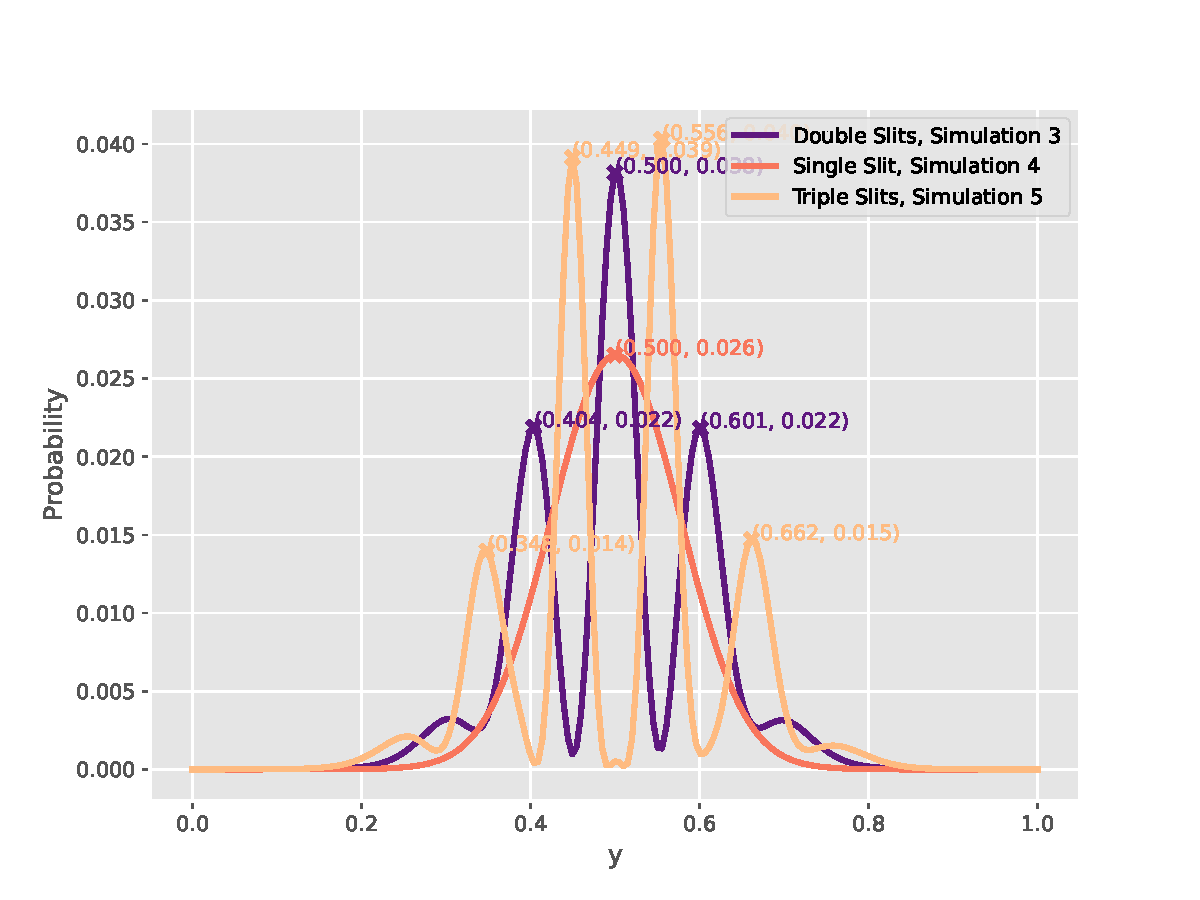
\includegraphics[width = 0.55\textwidth]{figures/wall.pdf} 
    \label{fig:comparison}
\end{figure}



\section{Discussion}\label{sec:discussion}
\subsection{No Barriers vs. Double Slits}
Figure \ref{fig:prob7} visualizes the deviation of the total probability from 1 as a function of time, for simulation of wave function behaviour with wall containing both no slits, and double slits in an interval of time $t\epsilon [0,0.008]$. From this figure, one can read an approximately constant difference between the two graphs, when both systems are evolved in time. Both the initial and final values for deviation for the system with no slits stay smaller than the system interacting with the wall containing double slits, something which  is explained by the extra work our machine has to do predicting the behaviour after reaction. Nonetheless, the two graphs display the same behaviour and shape, and indicates an increasing deviation as the simulation runs. The scale of this deviation, being as small as $10^{-14}$ and $10^{-15}$, further indicate a very small deviation either way, which can be grounds for the conclusion: the Figure \ref{fig:prob7} displays an abundance of correctness in our model. 



\subsection{Double Slits}
The Figure \ref{fig:doubleprob} visualizes the probability of measuring a Gaussian wave-packet at distinct positions in our well-defined environment with strict Dirichlet boundary conditions and double slits, at three different times t=0, t=0.001 and t=0.002. The Figures \ref{fig:doubleprobre} and \ref{fig:doubleprobim} show the same plots, divided into real and imaginary dimensions, for the same steps in time. \\

At t=0, the shape of the probability is centered around y=0.5, with a density with a Gaussian shape around this point. This is applicable to all three Figures, where we see clearly that the Figure \ref{fig:doubleprob} is a plot visualizing the sum of Figure \ref{fig:doubleprobre} and Figure \ref{fig:doubleprobim}. \\

From these three Figures combined, we can read a collision between the wave-function and the wall at time t=0.001. This, because our model works accurately, and only lets the wave-function pass through the modelled slits in the wall. The waves which are not passing through these slits are reflected when colliding with the wall as a consequence of the high potential. This pattern is clearly displayed in all three Figures at t=0.001, where reflection of half the wave-packets has taken place. \\

At t=0.002, some time has passed since the collision with the wall. The pattern we observe in the probability density, can be explained by the theory presented in section \ref{sec:behaviour}; the waves slipping through the slits in the wall, act according to Huygens principle, and expand in all directions within the xy-space with origins in the slits. Since there are two slits, the waves slipping through each of these will interact with each other, and in accordance with the superposition principle, result in interference occurring between them. \\

By taking a look at the 3D plot of the probability density at t=0.002, Figure \ref{fig:doubleprob3D}, one can obtain a clearer visualization of how exactly the density looks at this time. For the reflected waves, visualized as the probability in the interval $x\epsilon [0,0.5]$, the density is centered around two distinct peaks. These peaks are explained by interference as result of the \textit{"missing"} waves - the waves that slipped through the slits during interaction. In the rest of the interval in xy-space, $x\epsilon [0.5,1]$, we observe a density in probability for the waves moving through the slits, centered around a single point in space. This behaviour is also explained by the occurrence of interference between these waves. The simulation has placed the two slits along the y-axis, with an equal distance from the center y=0.5. This results in an constructive interference around the center itself, and destructive interference occurring in the intervals along the y-axis outside of our slits. \\

Thus, interference takes place in both the environment visualizing the reflected waves, and the waves passing through the slits. This occurrence of interference is as expected, and a result of the wave-particle duality our wave-packets possess. \\

The GIF \ref{gif:double} visualizing the simulation, linked in the Appendix \ref{sec:appendix}, in the entire time interval, shows how the waves are reflected at the Dirichlet boundaries of our modelled environment, and due to destructive interference and reflection, becomes less and less "collected" as time passes. This practically means the probability of measuring wave-packets, or the particles which our wave-packets model, in a random place in the xy-dimension increases with time. \\


\subsection{Detection Probability on Screen}
Simulations for behaviour of the wave-functions when colliding with a wall containing single, double and triple slits are performed, and the data accumulated from these simulations are compared in a single Figure \ref{fig:comparison}. This Figure \ref{fig:comparison} shows the probability for discovering particles along the y-axis at position x=0.8 and time t=0.002. We notice that the graphs for one slit has a single peak, the graph for double slits has three peaks, and the graph for triple slits has four peaks, all centered around the point y = 0.5. The point x=0.8 is placed behind the wall, so that the waves have to pass through the slits in order to reach it. Thereby, as we reflected upon previously, interference between the waves passing through the slits will be the cause of a pattern in the probability density. This is the reason we notice peaks in the graphs in Figure \ref{fig:comparison}. The three graphs have approximately the same shape, but peaks different amounts of times based on how may slits the wave-packets passes through. This pattern is reflected in the Figure \ref{fig:doubleprob}, where we can see the probability density reflected by the contour around y=0.5. \\

By taking another look at the Figure \ref{fig:doubleprob3D}, and expanding on our explanation of the behaviour occurring in this instance, the pattern of peaks in the Figure \ref{fig:comparison} can be explained easily. In all cases of splits - one, double and triple - all slits ace centered around the middle of our strictly defined xy-space. As for constructive interference occurring around y=0.5 in the instance of double slits, destructive interference will occur for the case of triple slits around the same y-coordinate. This is due to the third slit being placed with its centre at exactly y=0.5, to uphold the symmetry in our system. This further explains the amounts of peaks transpiring as well - these peaks will only be allowed to form where the constructive interference is the largest. In the case of a single slit, there will be no opportunity for wave-interactions, and the wave will behave in accordance with the Huygens principle, and expand in the xy-space, until reflected by the boundaries of our system, and wave-interactions again become pertinent.


\section{Conclusion}\label{sec:conclusion}
A model for the behaviour of wave-functions in a strictly defined, two dimensional space with Dirichlet boundary conditions was constructed. By making use of the Crank-Nicolson Scheme for partial difference equations, in combination with the two-dimensional time dependent Schrödinger equation, we managed to simulate the behaviour of a stream of particles, photons, described by the wave function for a Gaussian wave-packet. Using this model to simulate collisions between the wave function, and a wall with an arbitrary amount of slits constructed by defining a potential for the system, we visualized the probability density for the system at different moments in time. This probability density has the physical interpretation of probability of finding a particle with behaviour modelled by the wave function at a given position in the xy-space at the time t. \\

By simulating the behaviour of interactions between these waves, and a wall containing single, double and triple slits centered around y=0.5, a pattern of behaviour is displayed. By examining both figures and GIFs constructed from data accumulated by these simulations, we notice that the behaviour exhibited by the wave functions, is explained by the wave-particle duality, and we thereby prove that particles possess wave-like properties and vise versa. By obtaining these results, we can further conclude that the approach we had to modelling the system, and by making use of the Crank-Nicolson Scheme to evolve the system in time, was appropriate and garnered appropriate, accurate results. 




\bibliography{references.bib}{}
\bibliographystyle{plain}
\cleardoublepage
\section{Appendix}\label{sec:appendix}
\subsection{GIF Links}\label{sec:links}
Wall containing two slits, with variable-settings $h = 0.005$, $\Delta t = 2.5\times10^{-5}$, $T = 0.008$, $x_c = 0.25$, $\sigma_x = 0.05$, $p_x = 200$, $y_c = 0.5$, $\sigma_y = 0.05$, $p_y = 0$ and $v_0 = 0$. Thereby, the system is modelled two slits, with $v_0 = 1\times10^{10}$ and $\sigma_y = 0.10$ to simulating the behaviour of the wave-function: \\

\href{https://imgur.com/Tks8wPm}{Double slit}\label{gif:double} (https://imgur.com/Tks8wPm)\\

\textbf{Time intervals $t\epsilon [0,0.002]$}:\\
Wall containing single, double and triple slits, and environment defined by variables $h = 0.005$, $\Delta t = 2.5\times10^{-5}$, $T = 0.002$, $x_c = 0.25$, $\sigma_x = 0.05$, $p_x = 200$, $y_c = 0.5$, $\sigma_y = 0.20$, $p_y = 0$ and $v_0 = 1\times10^{10}$. Aperture is set to 0.05 and walls of length 0.05 in y-dimensions is used to separate the slits: \\
\href{https://imgur.com/vrzyZ6c}{Single slit}\label{gif:singlet}(https://imgur.com/vrzyZ6c)\\
\href{https://imgur.com/JNVzTY4}{Double slit}\label{gif:doublet}(https://imgur.com/JNVzTY4)\\
\href{https://imgur.com/cVFpt5g}{Triple slit}\label{gif:triplet}(https://imgur.com/cVFpt5g)\\

\href{https://imgur.com/a/3HzVBJA}{GIF} links to the imgur page containing all gifs created, visualizing  probability as a function of time (https://imgur.com/a/3HzVBJA).

\newpage
\subsection{Derivation of the Descretizised Schrödinger Equation}\label{sec:derivation}
We start with the Crank-Nicolson scheme for the time evolution of the wave function \(u\) in a two-dimensional space, Equation \eqref{eq:crank}, where \(F_{i,j}^n\) is given by Equation \eqref{eq:forward}, and \(F_{i,j}^{n+1}\) is given by Equation \eqref{eq:backward}. \\
These expressions can be inserted into the Equation \eqref{eq:crank}, and we get the expressions:
\[
\begin{aligned}
    &i \frac{u^{n+1}_{i,j}-u^{n}_{i,j}}{\Delta t} \\
    &= \frac{1}{2}(F_{i,j}^{n}+F_{i,j}^{n+1})\\
    &=\frac{1}{2}\left(i \frac{u^{n+1}_{i,j}-u^{n}_{i,j}}{\Delta t} \right. \\
    &- \left.\frac{u^n_{i+1,j}-2u^n_{i,j}+u^n_{i-1,j}}{h^2} - \frac{u^n_{i,j+1}-2u^n_{i,j}+u^n_{i,j-1} }{h^2} + u^n_{i,j}v_{i,j}\right.\\
    &+ \left.i \frac{u^{n+1}_{i,j}-u^{n}_{i,j}}{\Delta t} \right. \\
    &- \left.\frac{u^{n+1}_{i+1,j}- 2u^{n+1}_{i,j}+u^{n+1}_{i-1,j}}{h^2} - \frac{u^{n+1}_{i,j+1}-2u^{n+1}_{i,j}+u^{n+1}_{i,j-1} }{h^2} + u^{n+1}_{i,j}v_{i,j}\right)
\end{aligned}
\]
Now, define \(r = \frac{i \Delta t}{2h^2}\) and insert it into the equation:
\[
\begin{aligned}
    &i \frac{u^{n+1}_{i,j}-u^{n}_{i,j}}{\Delta t} \\
    &= r\left(u^n_{i+1,j}-2u^n_{i,j}+u^n_{i-1,j} + u^n_{i,j+1}-2u^n_{i,j}+u^n_{i,j-1} - 2u^n_{i,j}v_{i,j}\right)\\
    &+ r\left(u^{n+1}_{i+1,j}-2u^{n+1}_{i,j}+u^{n+1}_{i-1,j} + u^{n+1}_{i,j+1}-2u^{n+1}_{i,j}+u^{n+1}_{i,j-1} - 2u^{n+1}_{i,j}v_{i,j}\right)
\end{aligned}
\]
Now, simplify and rearrange the terms to obtain the discretized Schrödinger equation:
\[
\begin{aligned}
    &u_{ij}^{n+1} - r\left[u_{i+1,j}^{n+1} - 2u_{ij}^{n+1} + u_{i-1,j}^{n+1}\right] \\
    &- r\left[u_{i,j+1}^{n+1} - 2u_{ij}^{n+1} + u_{i,j-1}^{n+1}\right] + r v_{i,j} u_{ij}^{n+1} \\
    &= u_{ij}^n + r\left[u_{i+1,j}^n - 2u_{ij}^n + u_{i-1,j}^n\right] \\
    &+ r\left[u_{i,j+1}^n - 2u_{ij}^n + u_{i,j-1}^n\right] - r v_{i,j} u_{ij}^n.
\end{aligned}
\]
%\vspace*{100\baselineskip}
\end{document}